\def\retinafocusresults{
    Một đặc điểm của mô hình RetinaFocus là có nhiều cấu hình có thể cài đặt để triển khai mô hình như cấu hình lựa chọn bản đồ đặc trưng\index{bản đồ đặc trưng} của FPN cho nhánh tập trung đối tượng\index{nhánh tập trung đối tượng}, cấu hình scale ảnh trong quá trình dự đoán \dots
    Vì vậy, ta cần so sánh và lựa chọn cấu hình tối ưu nhất, cân đối giữa thời gian thực hiện quá trình dự đoán và độ chính xác của mô hình.
    Để so sánh một cách toàn diện nhất, ta sẽ sử dụng cả hai bộ dữ liệu WIDER FACE thông thường và bộ dữ liệu WIDER FACE kích thước lớn.

    \subsubsection*{Thí nghiệm so sánh các cấu hình sử dụng bản đồ đặc trưng\index{bản đồ đặc trưng} khác nhau của FPN làm đầu vào cho nhánh tập trung đối tượng}
    Trong thí nghiệm này, với mỗi cấu hình, chúng tôi sử dụng các bản đồ đặc trưng\index{bản đồ đặc trưng} khác nhau của FPN làm đầu vào cho nhánh tập trung đối tượng\index{nhánh tập trung đối tượng}.
    Trong đó, lần lượt các cấu hình sử dụng bản đồ đặc trưng\index{bản đồ đặc trưng} ${C}_{3}, {C}_{4}, {C}_{5}, {P}_{3}, {P}_{4}, {P}_{5}$ được ký hiệu là \textit{using feature maps C3}, \textit{using feature maps C4}, \textit{using feature maps C5}, \textit{using feature maps P3}, \textit{using feature maps P4}, \textit{using feature maps P5} trong các biểu đồ.
    Trong các cấu hình trên, các cặp bản đồ đặc trưng\index{bản đồ đặc trưng} ${C}_{3}$ và ${P}_{3}$, ${C}_{4}$ và ${P}_{4}$, ${C}_{5}$ và ${P}_{5}$ là các cặp bản đồ đặc trưng\index{bản đồ đặc trưng} có cùng kích thước.
    Tuy nhiên, mỗi bản đồ đặc trưng\index{bản đồ đặc trưng} khác nhau trong cặp chứa thông tin khác nhau về khuôn mặt dẫn đến số lượng và kích thước của các vùng mà nhánh tập trung đối tượng\index{nhánh tập trung đối tượng} xác định cần phải zoom vào cũng khác nhau.
    Từ đó dẫn đến thời gian thực hiện toàn bộ quá trình dự đoán trên cả bộ dữ liệu là khác nhau.
    % Trong thí nghiệm này, các cấu hình sử dụng chung một cấu hình scale ảnh trong quá trình dự đoán là ....

    \begin{figure}[H]
        \centering
        \subfigure[]{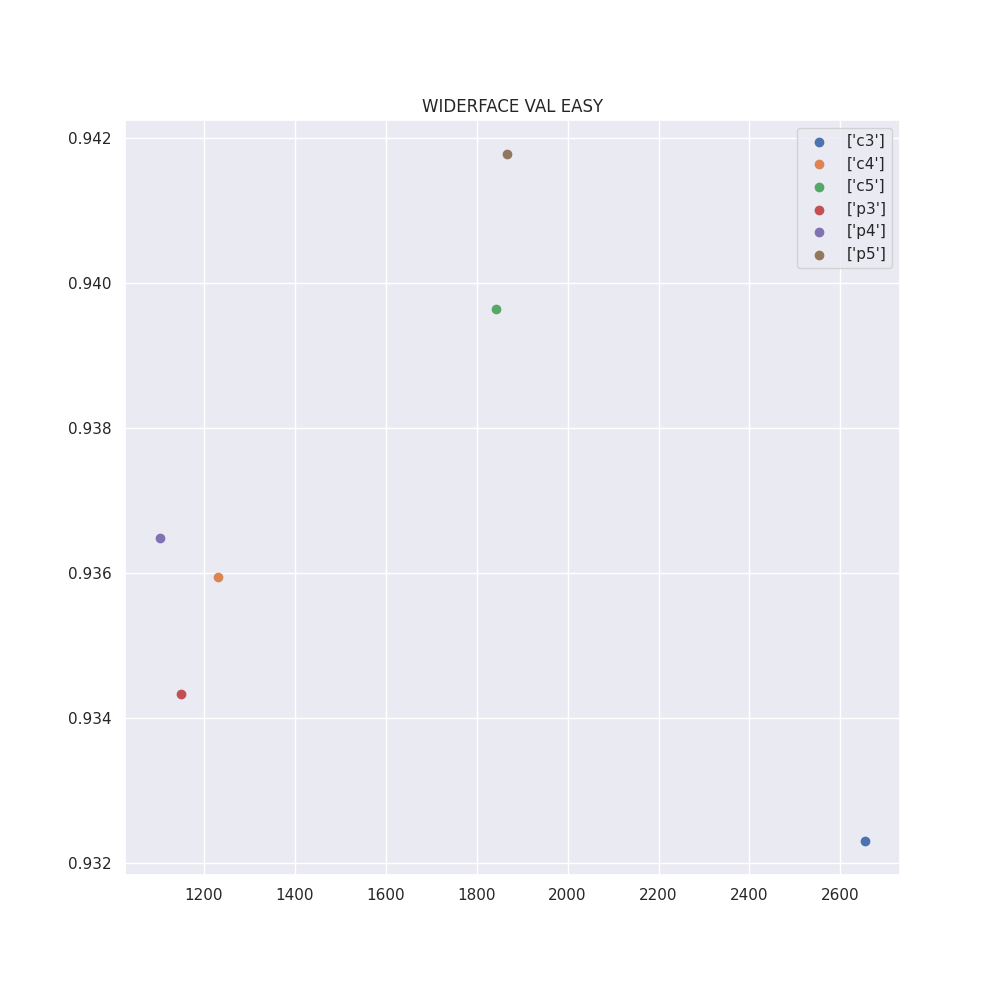
\includegraphics[width=7.3cm]{images/retinafocus_widerface_val_easy_fpn}} 
        \subfigure[]{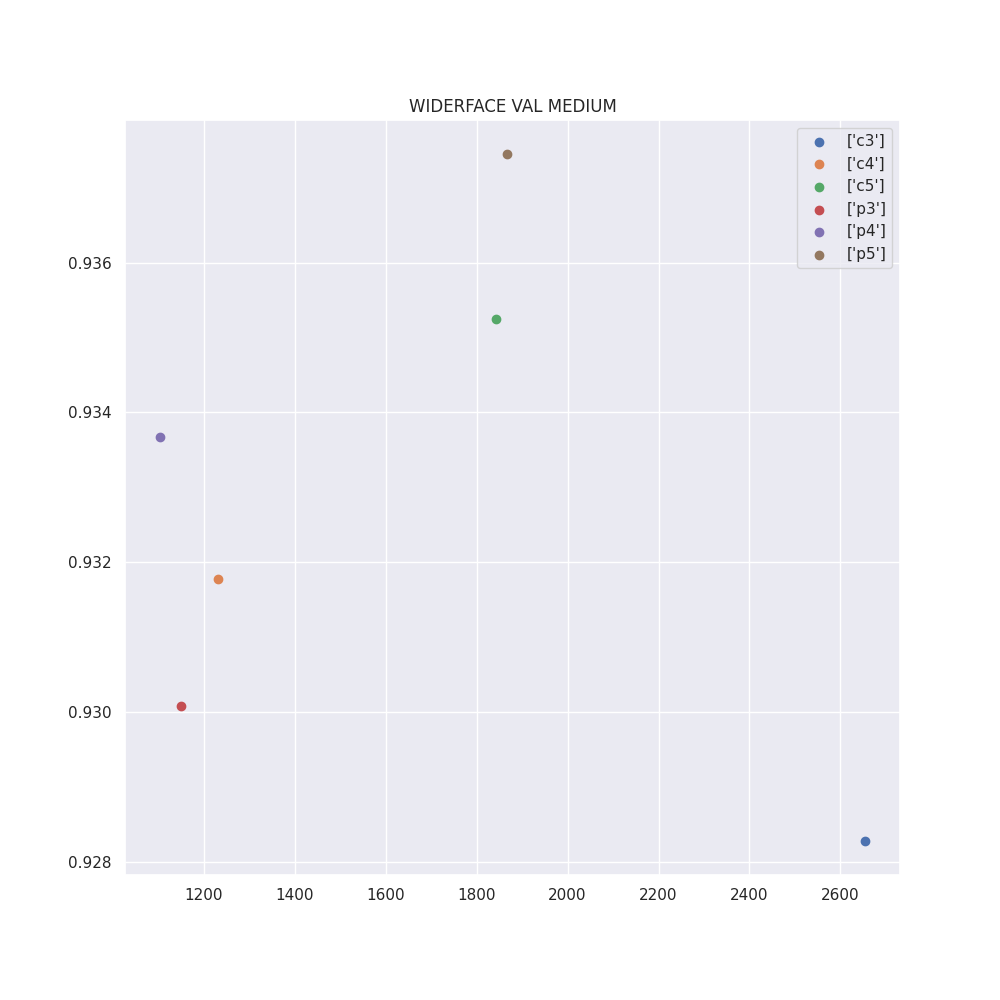
\includegraphics[width=7.3cm]{images/retinafocus_widerface_val_medium_fpn}} 
        \subfigure[]{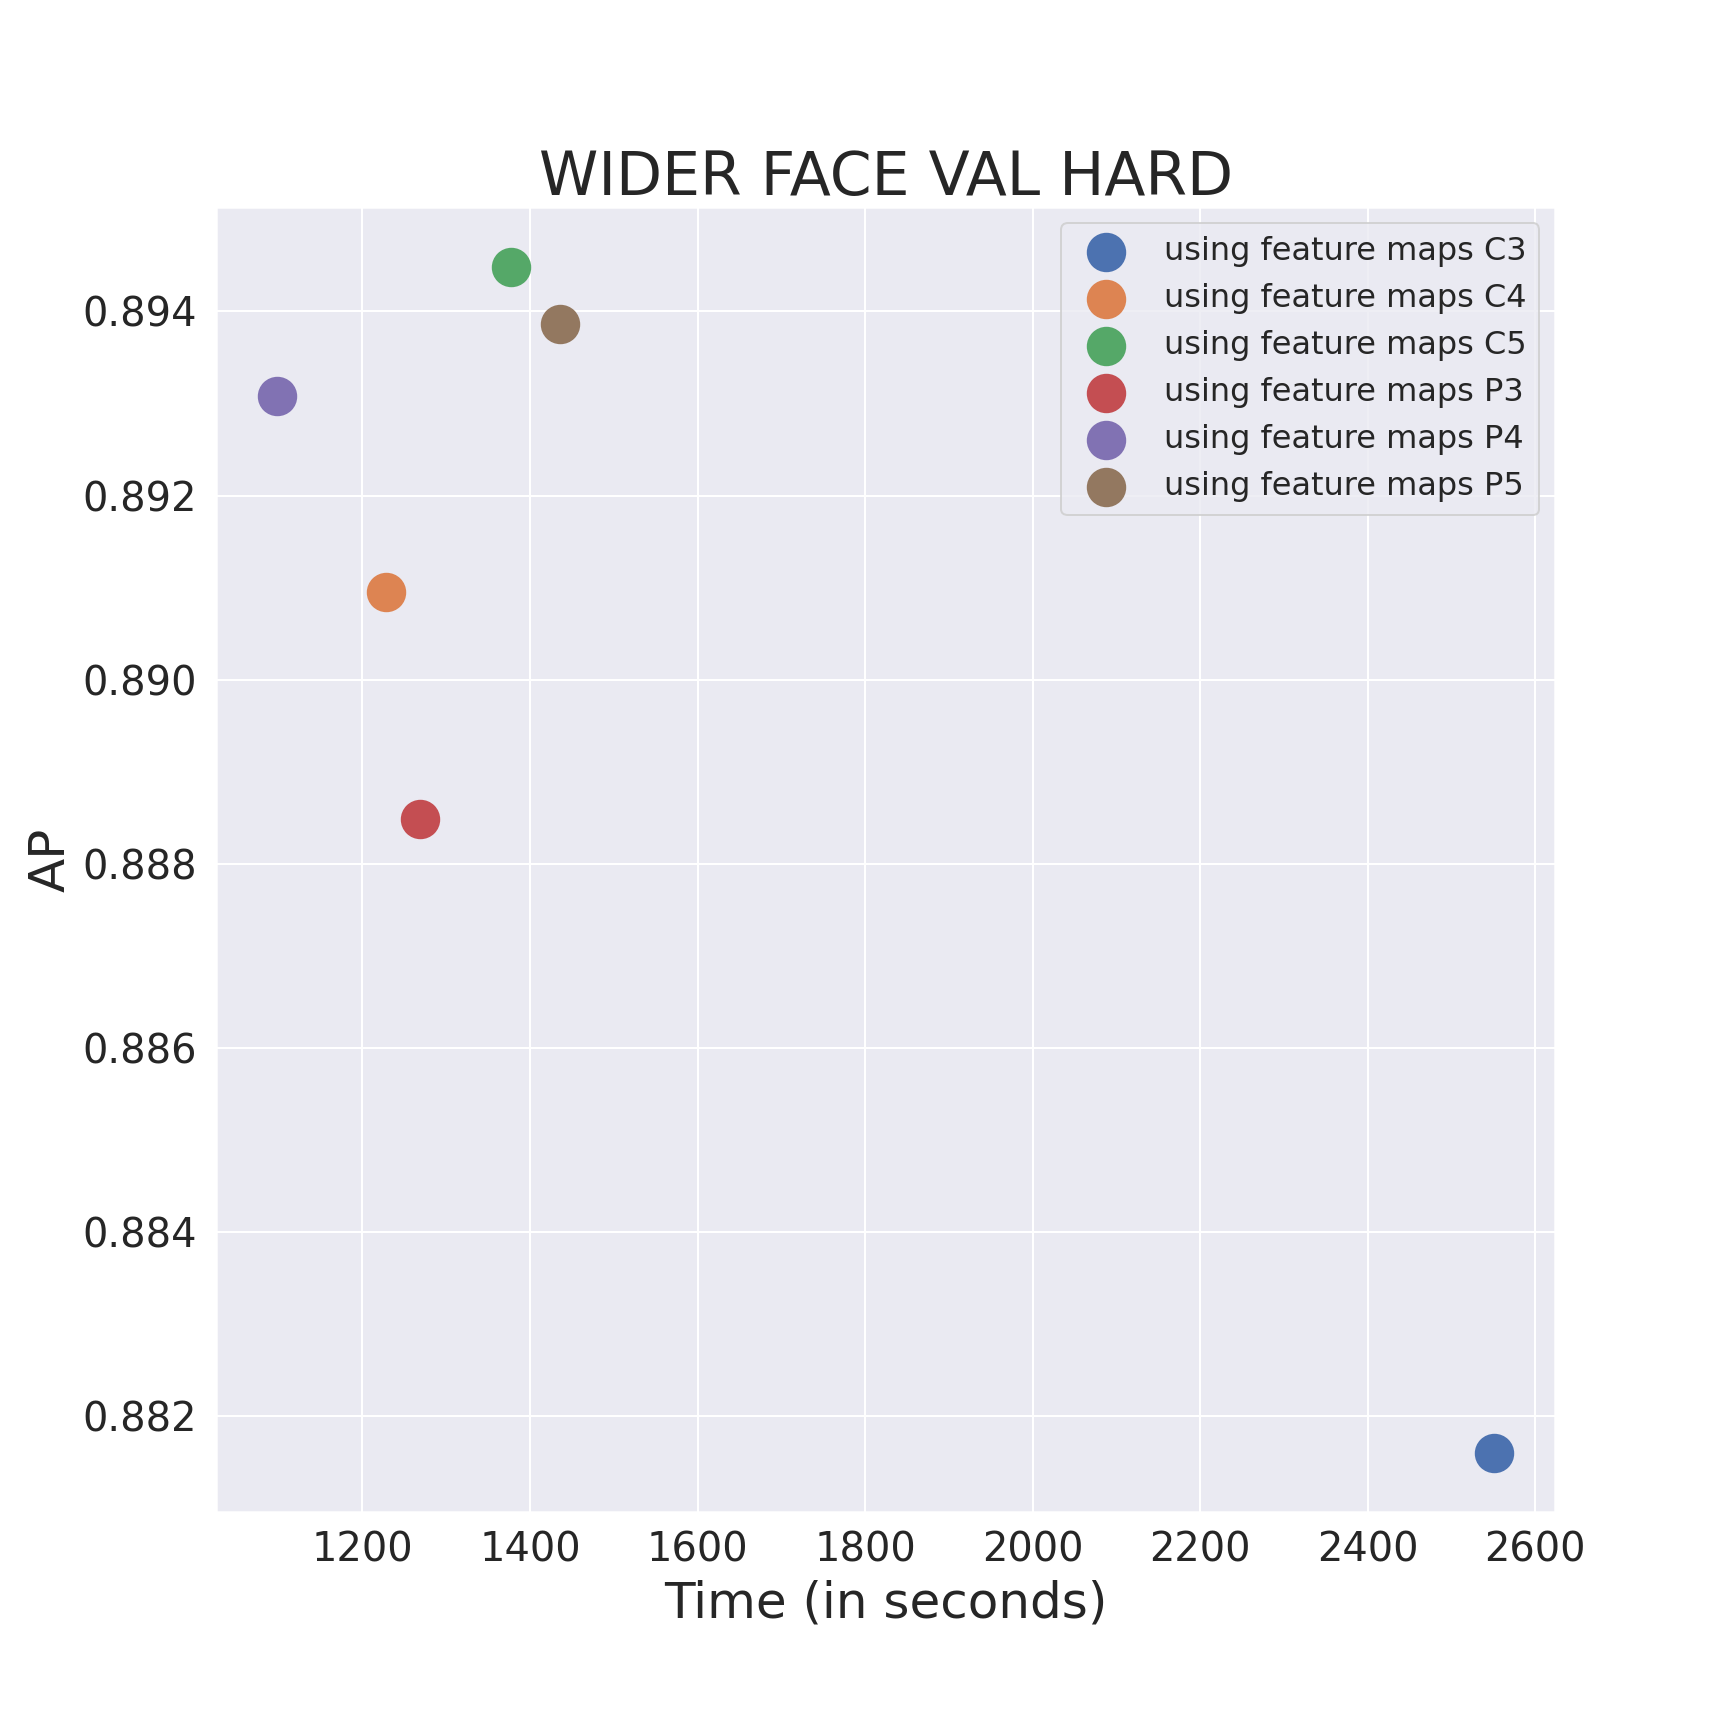
\includegraphics[width=7.3cm]{images/retinafocus_widerface_val_hard_fpn}} 
        \caption{Kết quả so sánh các cấu hình sử dụng các bản đồ đặc trưng\index{bản đồ đặc trưng} của FPN làm đầu vào cho nhánh tập trung đối tượng\index{nhánh tập trung đối tượng} trên ba bộ dữ liệu WIDER FACE val easy (a), medium (b) và hard (c)}
        \label{fig:retinafocus_widerface_val_fpn}
    \end{figure}

    \noindent
    Đối với bộ WIDER FACE thông thường, hai cấu hình đạt độ chính xác cao nhất là cấu hình sử dụng bản đồ đặc trưng\index{bản đồ đặc trưng} ${P}_{5}$ và cấu hình sử dụng bản đồ đặc trưng\index{bản đồ đặc trưng} ${C}_{5}$ cho nhánh tập trung đối tượng\index{nhánh tập trung đối tượng} với thời gian thực hiện toàn bộ quá trình dự đoán trên cả bộ dữ liệu lần lượt là 1436 và 1377 giây.
    Trong khi cấu hình sử dụng bản đồ đặc trưng\index{bản đồ đặc trưng} ${P}_{5}$ cho kết quả tốt hơn trên bộ WIDER FACE val easy và medium thì cấu hình sử dụng bản đồ đặc trưng\index{bản đồ đặc trưng} ${C}_{5}$ cho kết quả tốt hơn trên bộ WIDER FACE val hard.
    Các cấu hình khác như ${P}_{4}$, ${P}_{3}$ và ${C}_{4}$ có thời gian thực hiện toàn bộ quá trình dự đoán nhanh hơn nhưng độ chính xác không tốt.
    Đặc biệt là cấu hình ${C}_{3}$ vừa có thời gian thực hiện toàn bộ quá trình dự đoán chậm vừa đạt độ chính xác thấp.

    \begin{figure}[H]
        \centering
        \subfigure[]{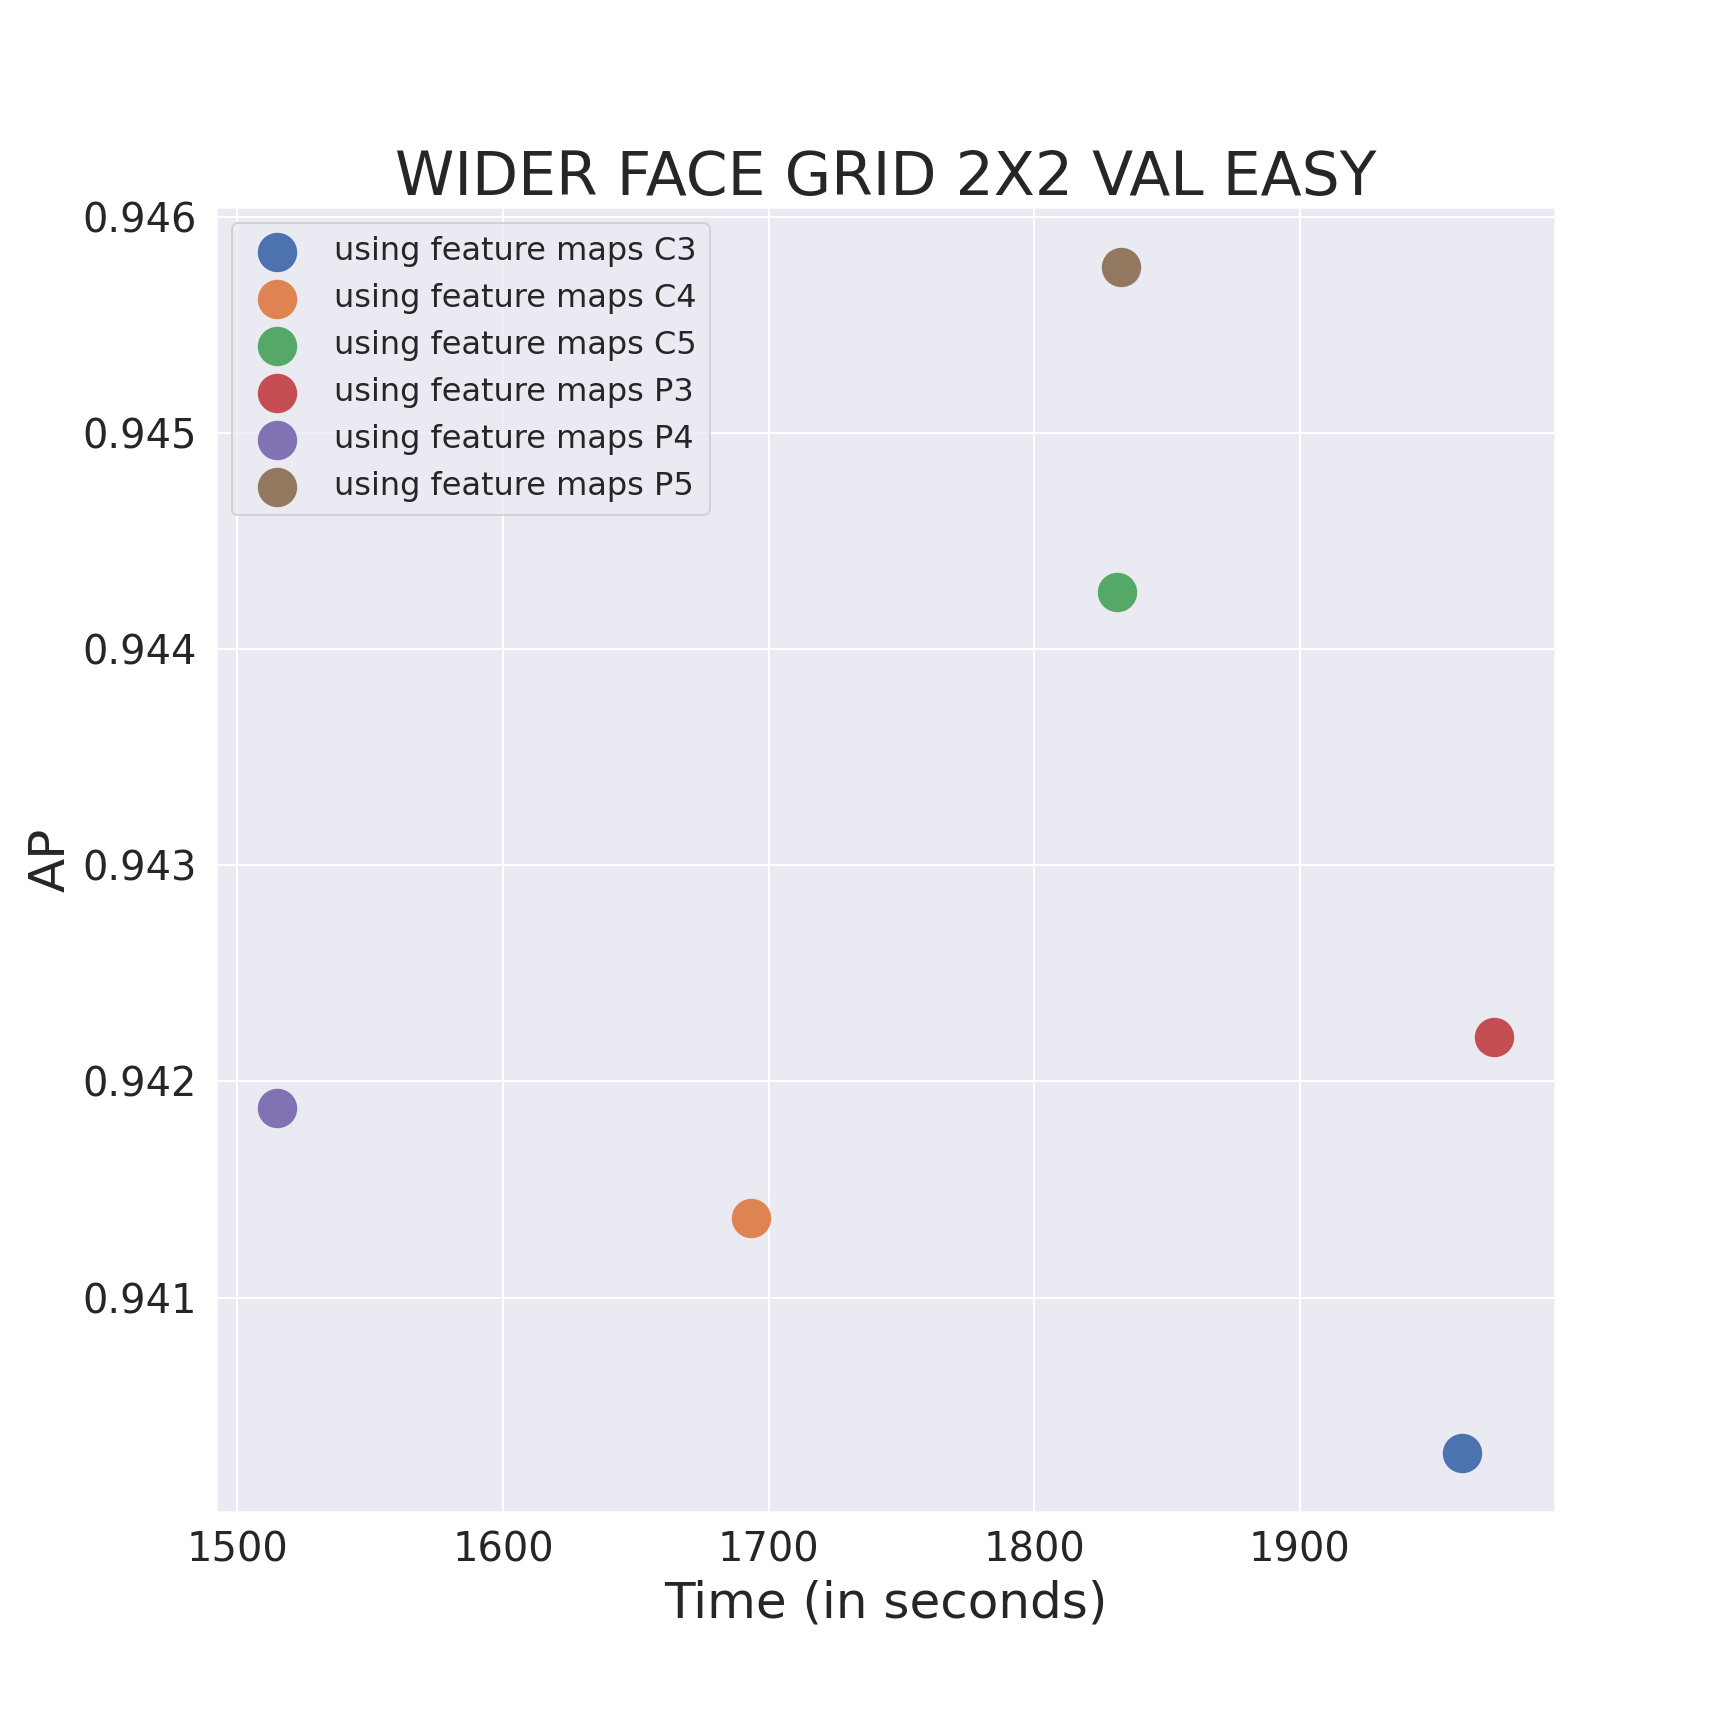
\includegraphics[width=7.3cm]{images/retinafocus_widerface_2k_val_easy_fpn}} 
        \subfigure[]{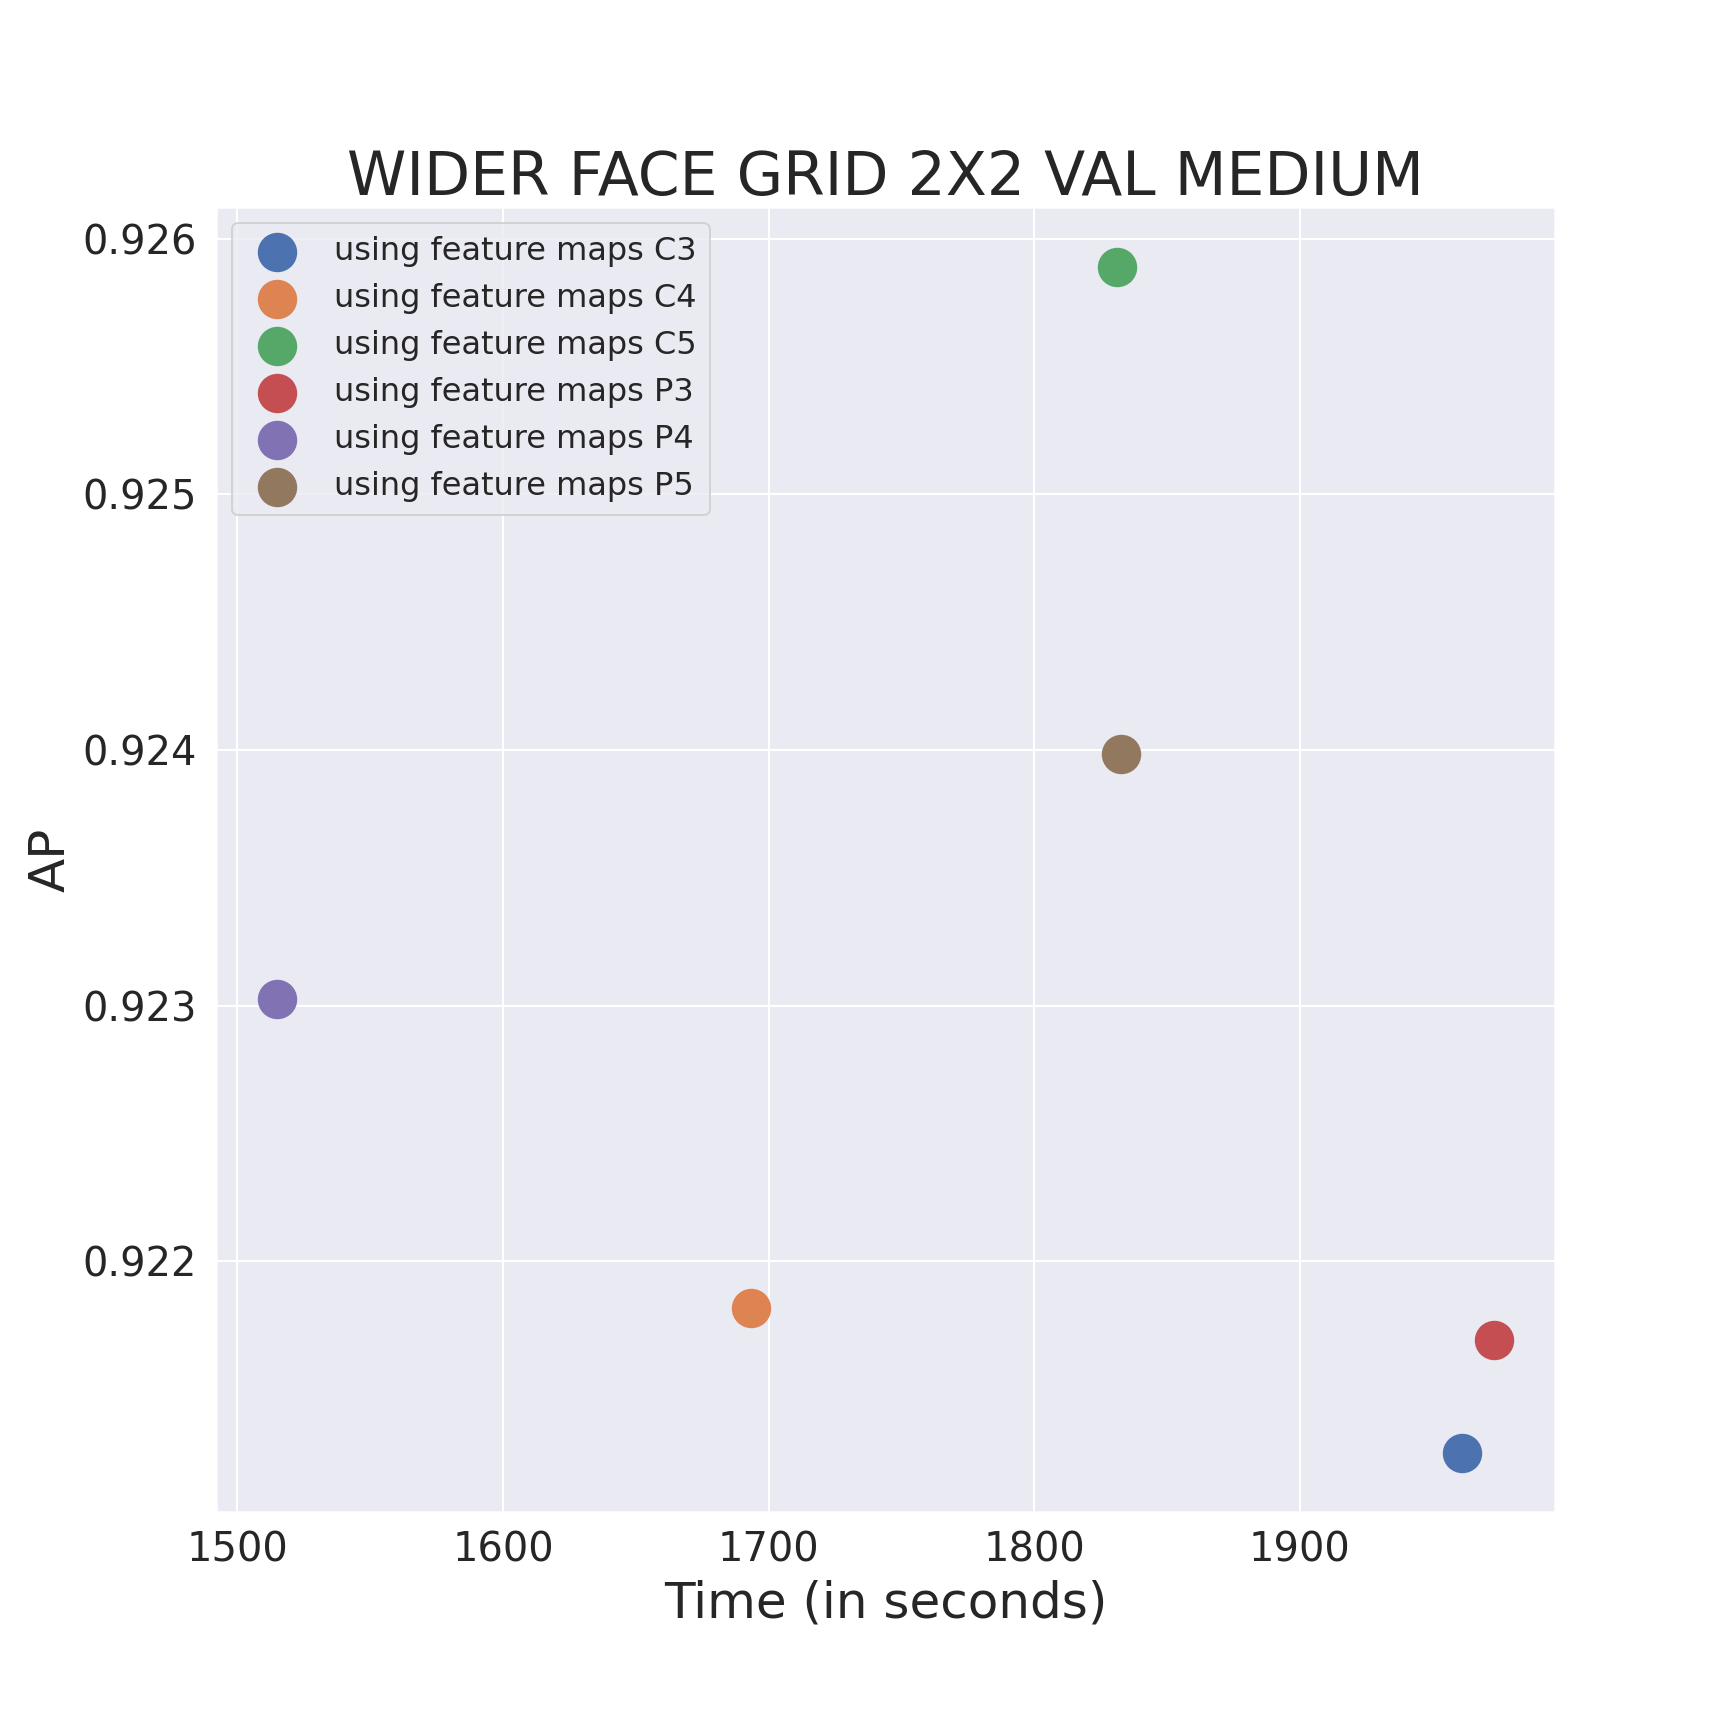
\includegraphics[width=7.3cm]{images/retinafocus_widerface_2k_val_medium_fpn}} 
        \subfigure[]{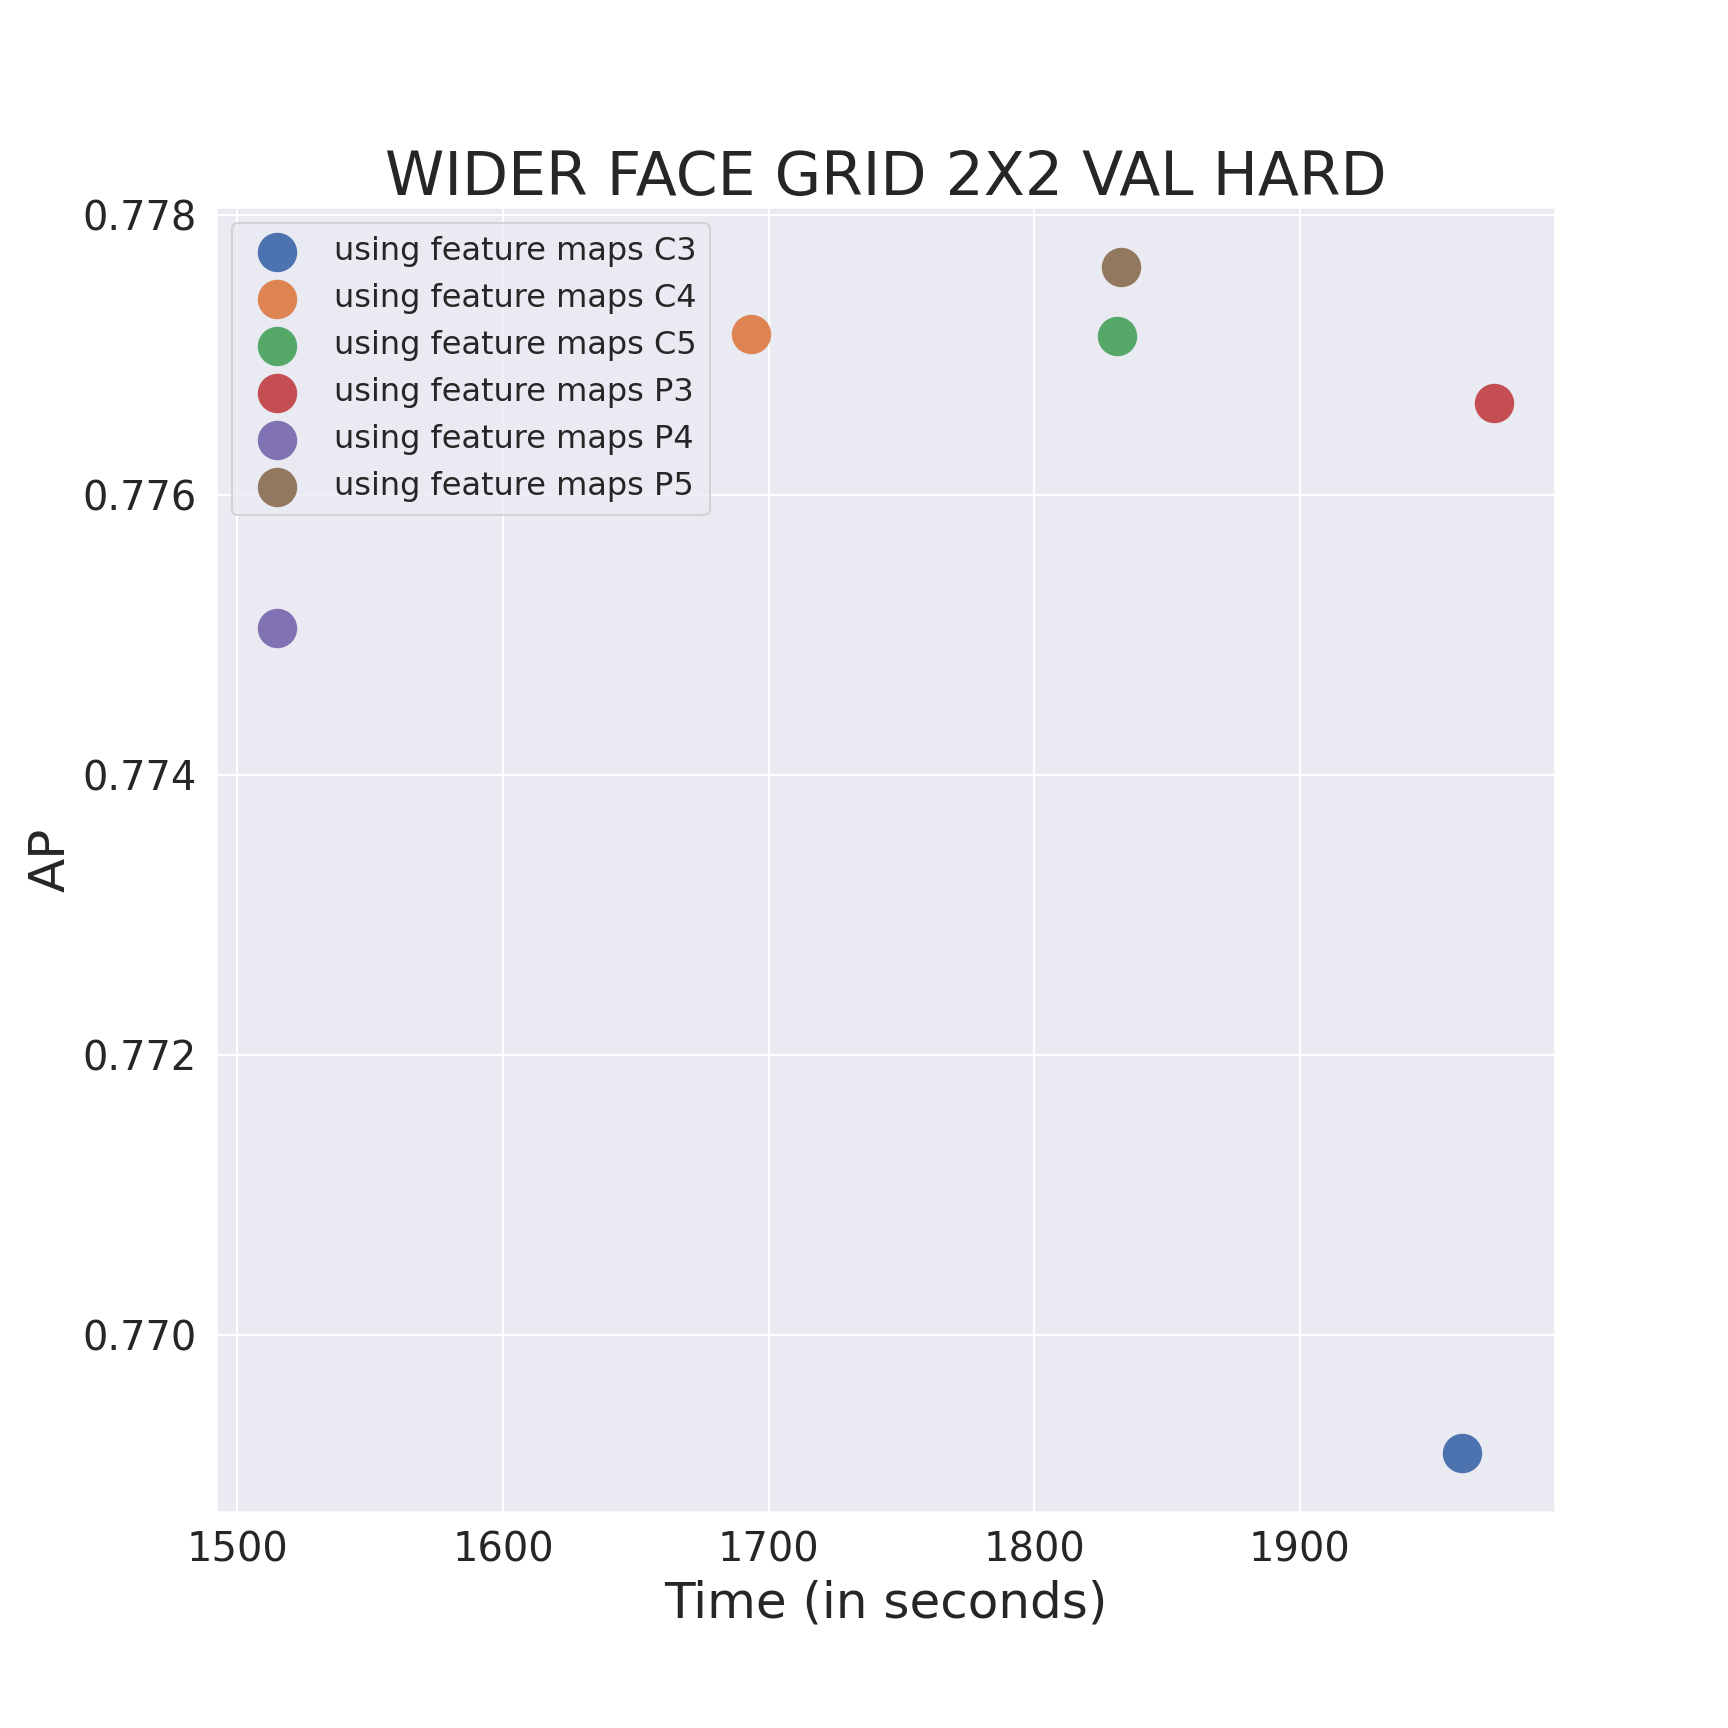
\includegraphics[width=7.3cm]{images/retinafocus_widerface_2k_val_hard_fpn}} 
        \caption{Kết quả so sánh các cấu hình sử dụng các bản đồ đặc trưng\index{bản đồ đặc trưng} của FPN làm đầu vào cho nhánh tập trung đối tượng\index{nhánh tập trung đối tượng} trên ba bộ dữ liệu WIDER FACE kích thước lớn lưới $2 \times 2$ val easy (a), medium (b) và hard (c)}
        \label{fig:retinafocus_widerface_4k_val_fpn}
    \end{figure}

    \noindent
    Đối với bộ WIDER FACE kích thước lớn lưới $2 \times 2$, hai cấu hình đạt độ chính xác cao nhất vẫn là cấu hình sử dụng bản đồ đặc trưng\index{bản đồ đặc trưng} ${P}_{5}$ và cấu hình sử dụng bản đồ đặc trưng\index{bản đồ đặc trưng} ${C}_{5}$ với thời gian thực hiện toàn bộ quá trình dự đoán trên cả bộ dữ liệu lần lượt là 1832 và 1831 giây.
    Đối với bộ dữ liệu này, trong khi cấu hình sử dụng bản đồ đặc trưng\index{bản đồ đặc trưng} ${P}_{5}$ cho kết quả tốt hơn trên bộ WIDER FACE kích thước lớn lưới $2 \times 2$ val easy và hard thì cấu hình sử dụng bản đồ đặc trưng\index{bản đồ đặc trưng} ${C}_{5}$ cho kết quả tốt hơn trên bộ WIDER FACE kích thước lớn lưới $2 \times 2$ val medium.
    Tuy nhiên, đối với bộ WIDER FACE kích thước lớn lưới $2 \times 2$ val hard, kết quả của cấu hình sử dụng bản đồ đặc trưng\index{bản đồ đặc trưng} ${C}_{4}$ và ${P}_{3}$ cho kết quả khá tiệm cận với cấu hình sử dụng bản đồ đặc trưng\index{bản đồ đặc trưng} ${C}_{5}$.

    \begin{figure}[H]
        \centering
        \subfigure[]{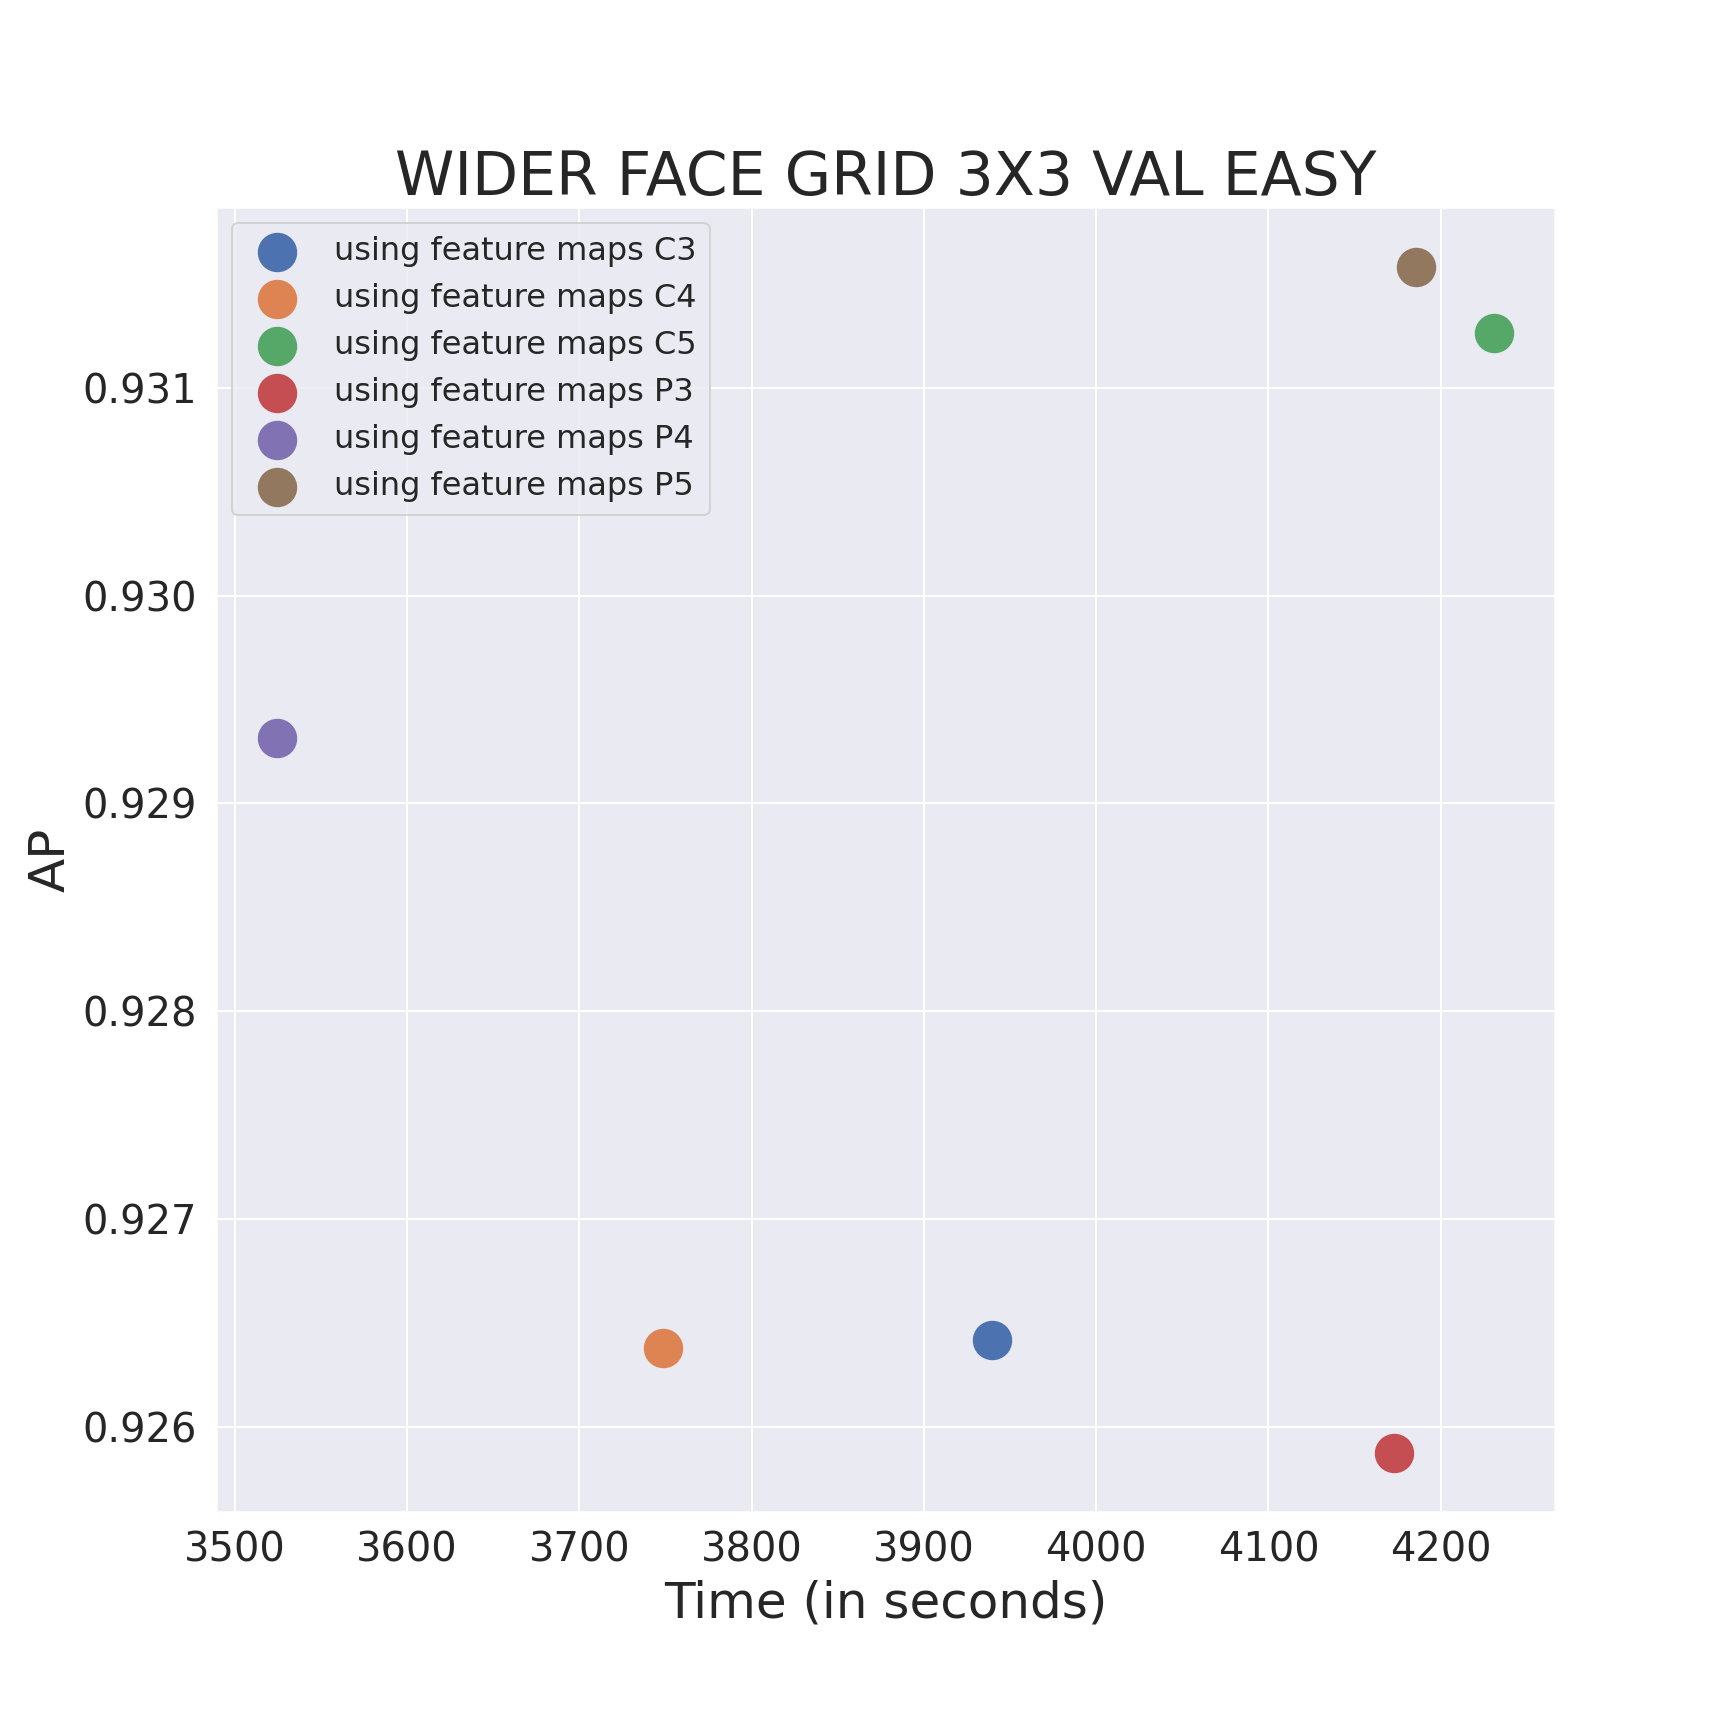
\includegraphics[width=7.3cm]{images/retinafocus_widerface_3k_val_easy_fpn}} 
        \subfigure[]{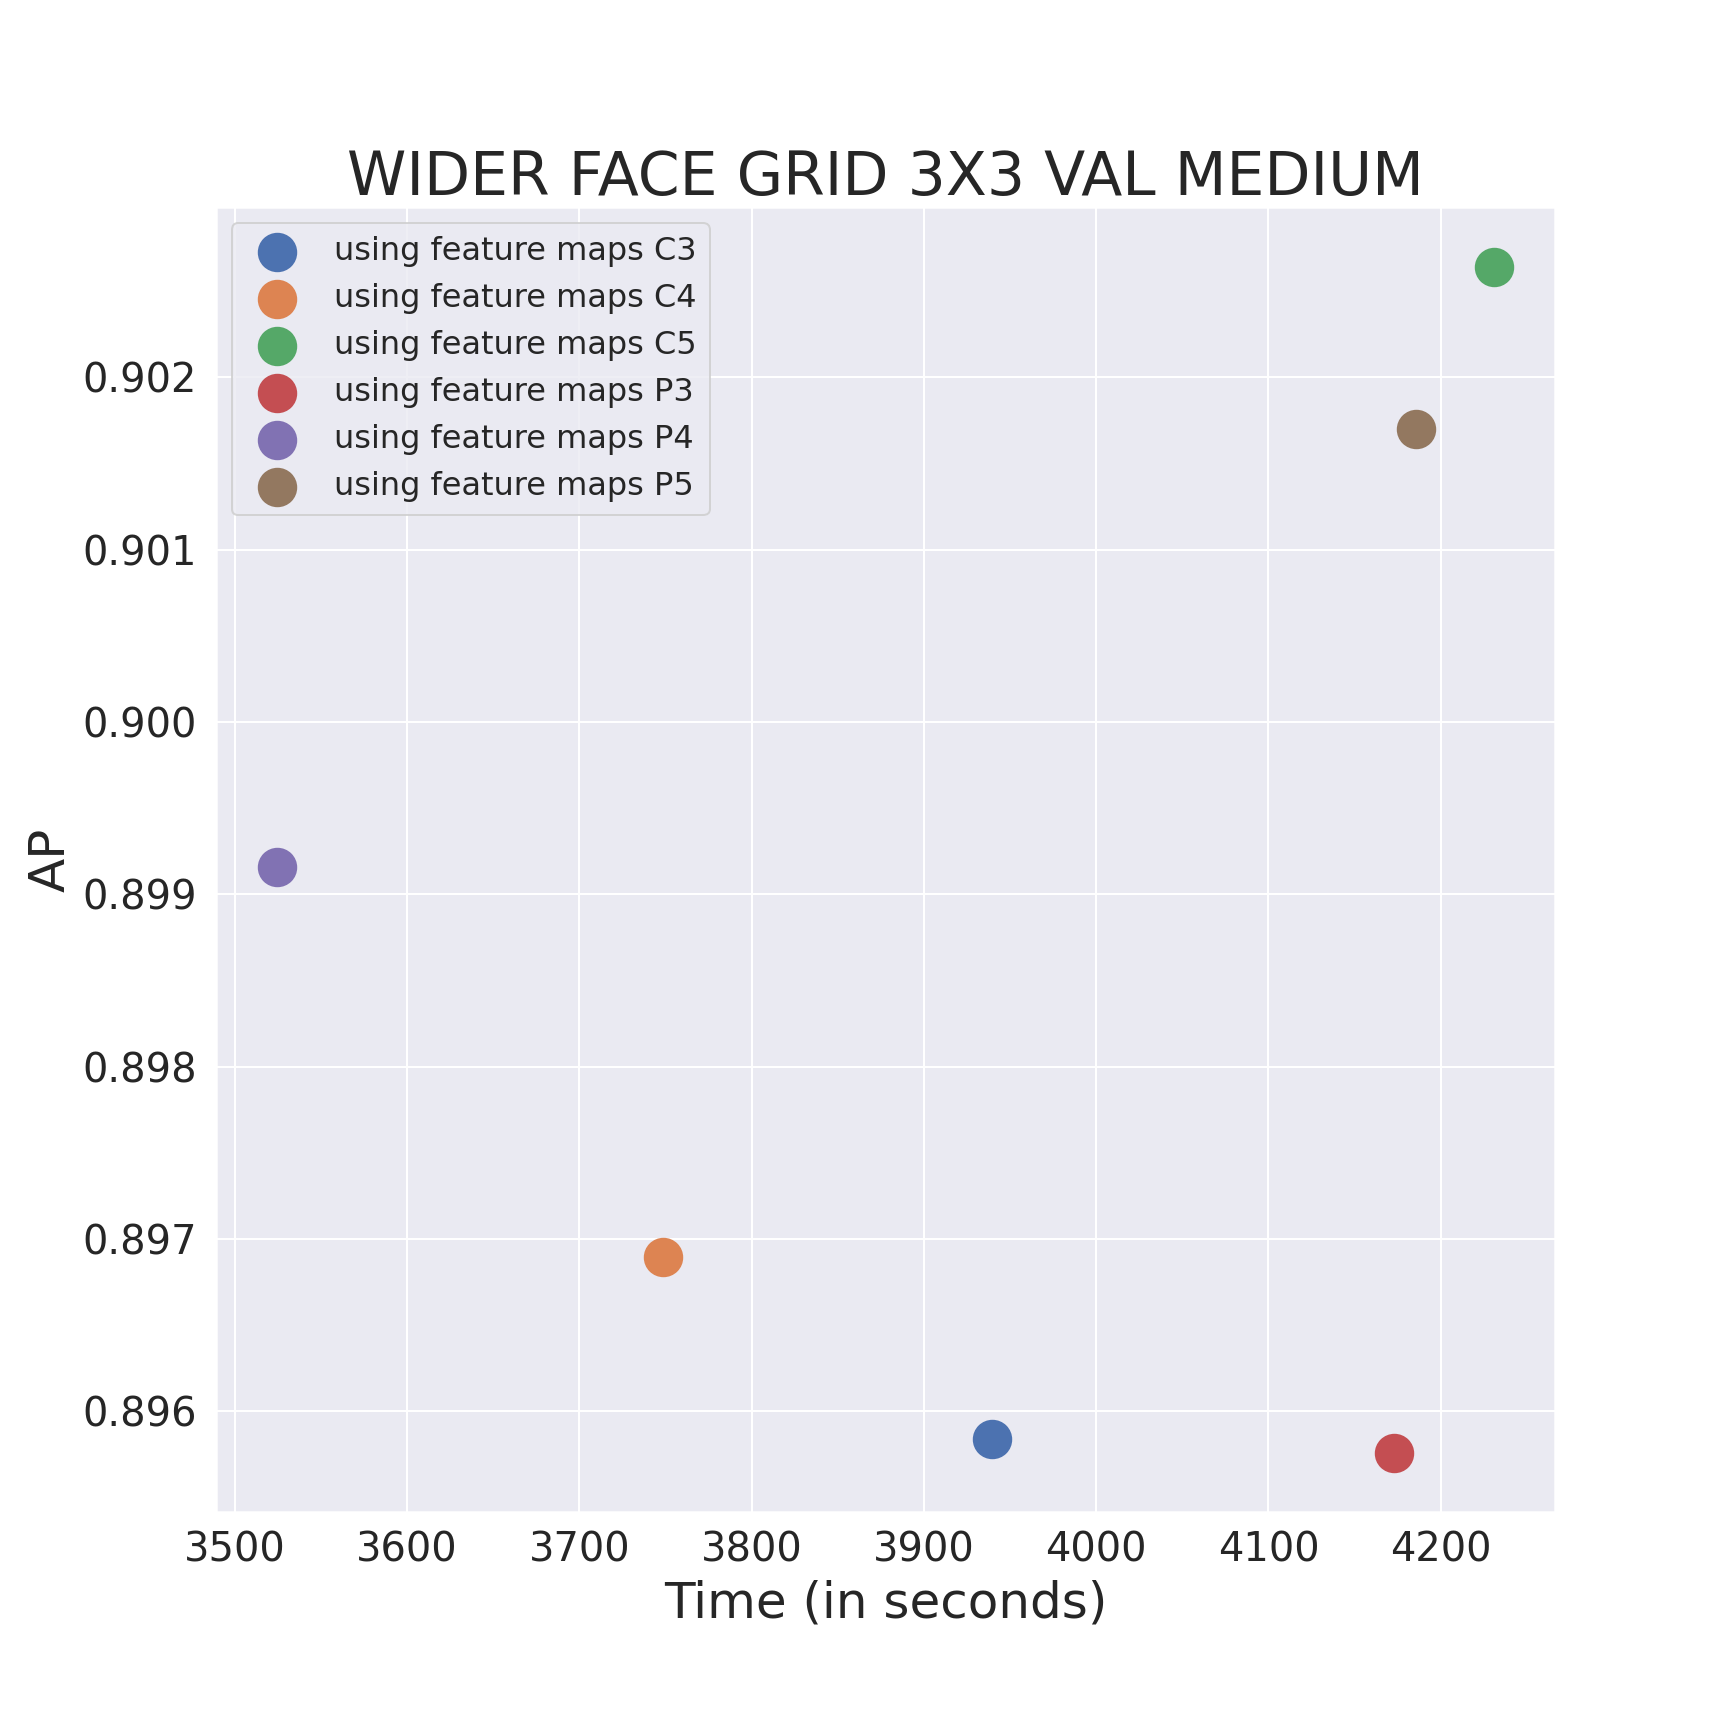
\includegraphics[width=7.3cm]{images/retinafocus_widerface_3k_val_medium_fpn}} 
        \subfigure[]{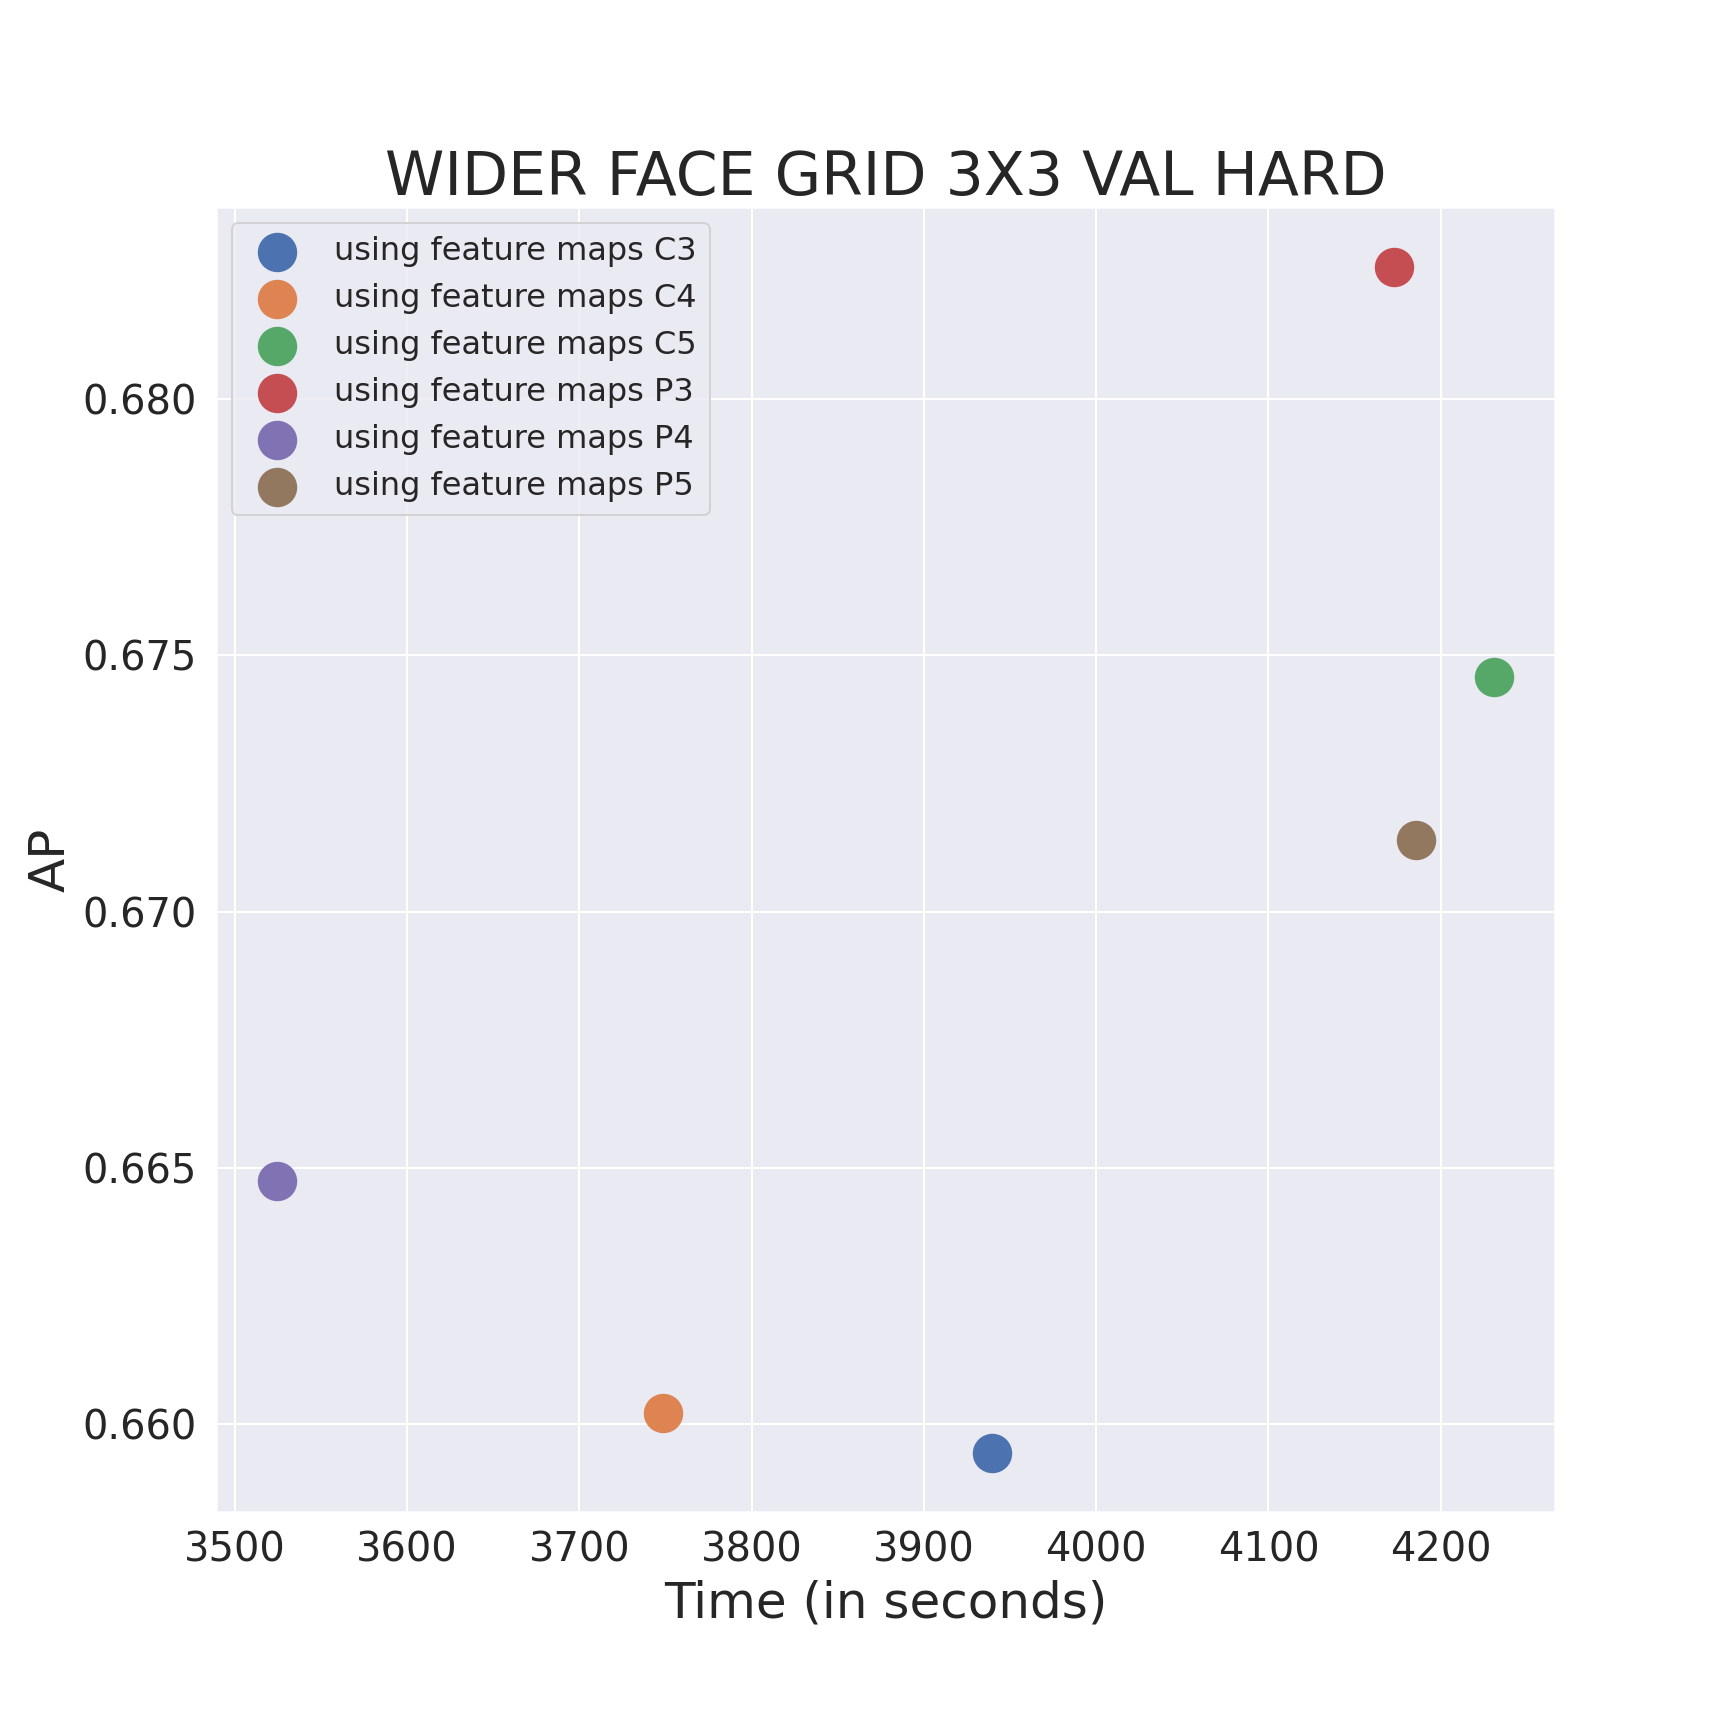
\includegraphics[width=7.3cm]{images/retinafocus_widerface_3k_val_hard_fpn}} 
        \caption{Kết quả so sánh các cấu hình sử dụng các bản đồ đặc trưng\index{bản đồ đặc trưng} của FPN làm đầu vào cho nhánh tập trung đối tượng\index{nhánh tập trung đối tượng} trên ba bộ dữ liệu WIDER FACE kích thước lớn lưới $3 \times 3$ val easy (a), medium (b) và hard (c)}
        \label{fig:retinafocus_widerface_4k_val_fpn}
    \end{figure}

    \noindent
    Đối với bộ WIDER FACE kích thước lớn lưới $3 \times 3$, các cấu hình đạt độ chính xác cao nhất đã có những sự thay đổi.
    Đối với bộ WIDER FACE kích thước lớn lưới $3 \times 3$ easy, cấu hình sử dụng bản đồ đặc trưng\index{bản đồ đặc trưng} ${P}_{5}$ cho kết quả tốt nhất với thời gian thực hiện toàn bộ quá trình dự đoán trên cả bộ dữ liệu lần lượt là 4185 giây.
    Đối với bộ WIDER FACE kích thước lớn lưới $3 \times 3$ medium, cấu hình sử dụng bản đồ đặc trưng\index{bản đồ đặc trưng} ${C}_{5}$ cho kết quả tốt nhất với thời gian thực hiện toàn bộ quá trình dự đoán trên cả bộ dữ liệu lần lượt là 4231 giây.
    Đối với bộ WIDER FACE kích thước lớn lưới $3 \times 3$ hard, cấu hình sử dụng bản đồ đặc trưng\index{bản đồ đặc trưng} ${P}_{3}$ cho kết quả tốt nhất, vượt qua khá xa hai cấu hình sử dụng bản đồ đặc trưng\index{bản đồ đặc trưng} ${P}_{5}$ và ${C}_{5}$, với thời gian thực hiện toàn bộ quá trình dự đoán trên cả bộ dữ liệu lần lượt là 4172 giây.

    \noindent
    Kết luận đối với thí nghiệm này, đối với mỗi bộ dữ liệu khác nhau như WIDER FACE thông thường, WIDER FACE kích thước lớn lưới $2 \times 2$ hay $3 \times 3$ và các bộ dữ liệu con easy, medium và hard, kết quả về cấu hình đạt độ chính xác cao nhất khác nhau, phụ thuộc vào kích thước ảnh đầu vào và tỷ lệ giữa kích thước của hộp giới hạn\index{hộp giới hạn} và kích thước của ảnh đầu vào tương ứng.

    \subsubsection*{Thí nghiệm so sánh cấu hình tốt nhất của RetinaFocus với các cấu hình của RetinaFace}

    \begin{figure}[H]
        \centering
        \subfigure[]{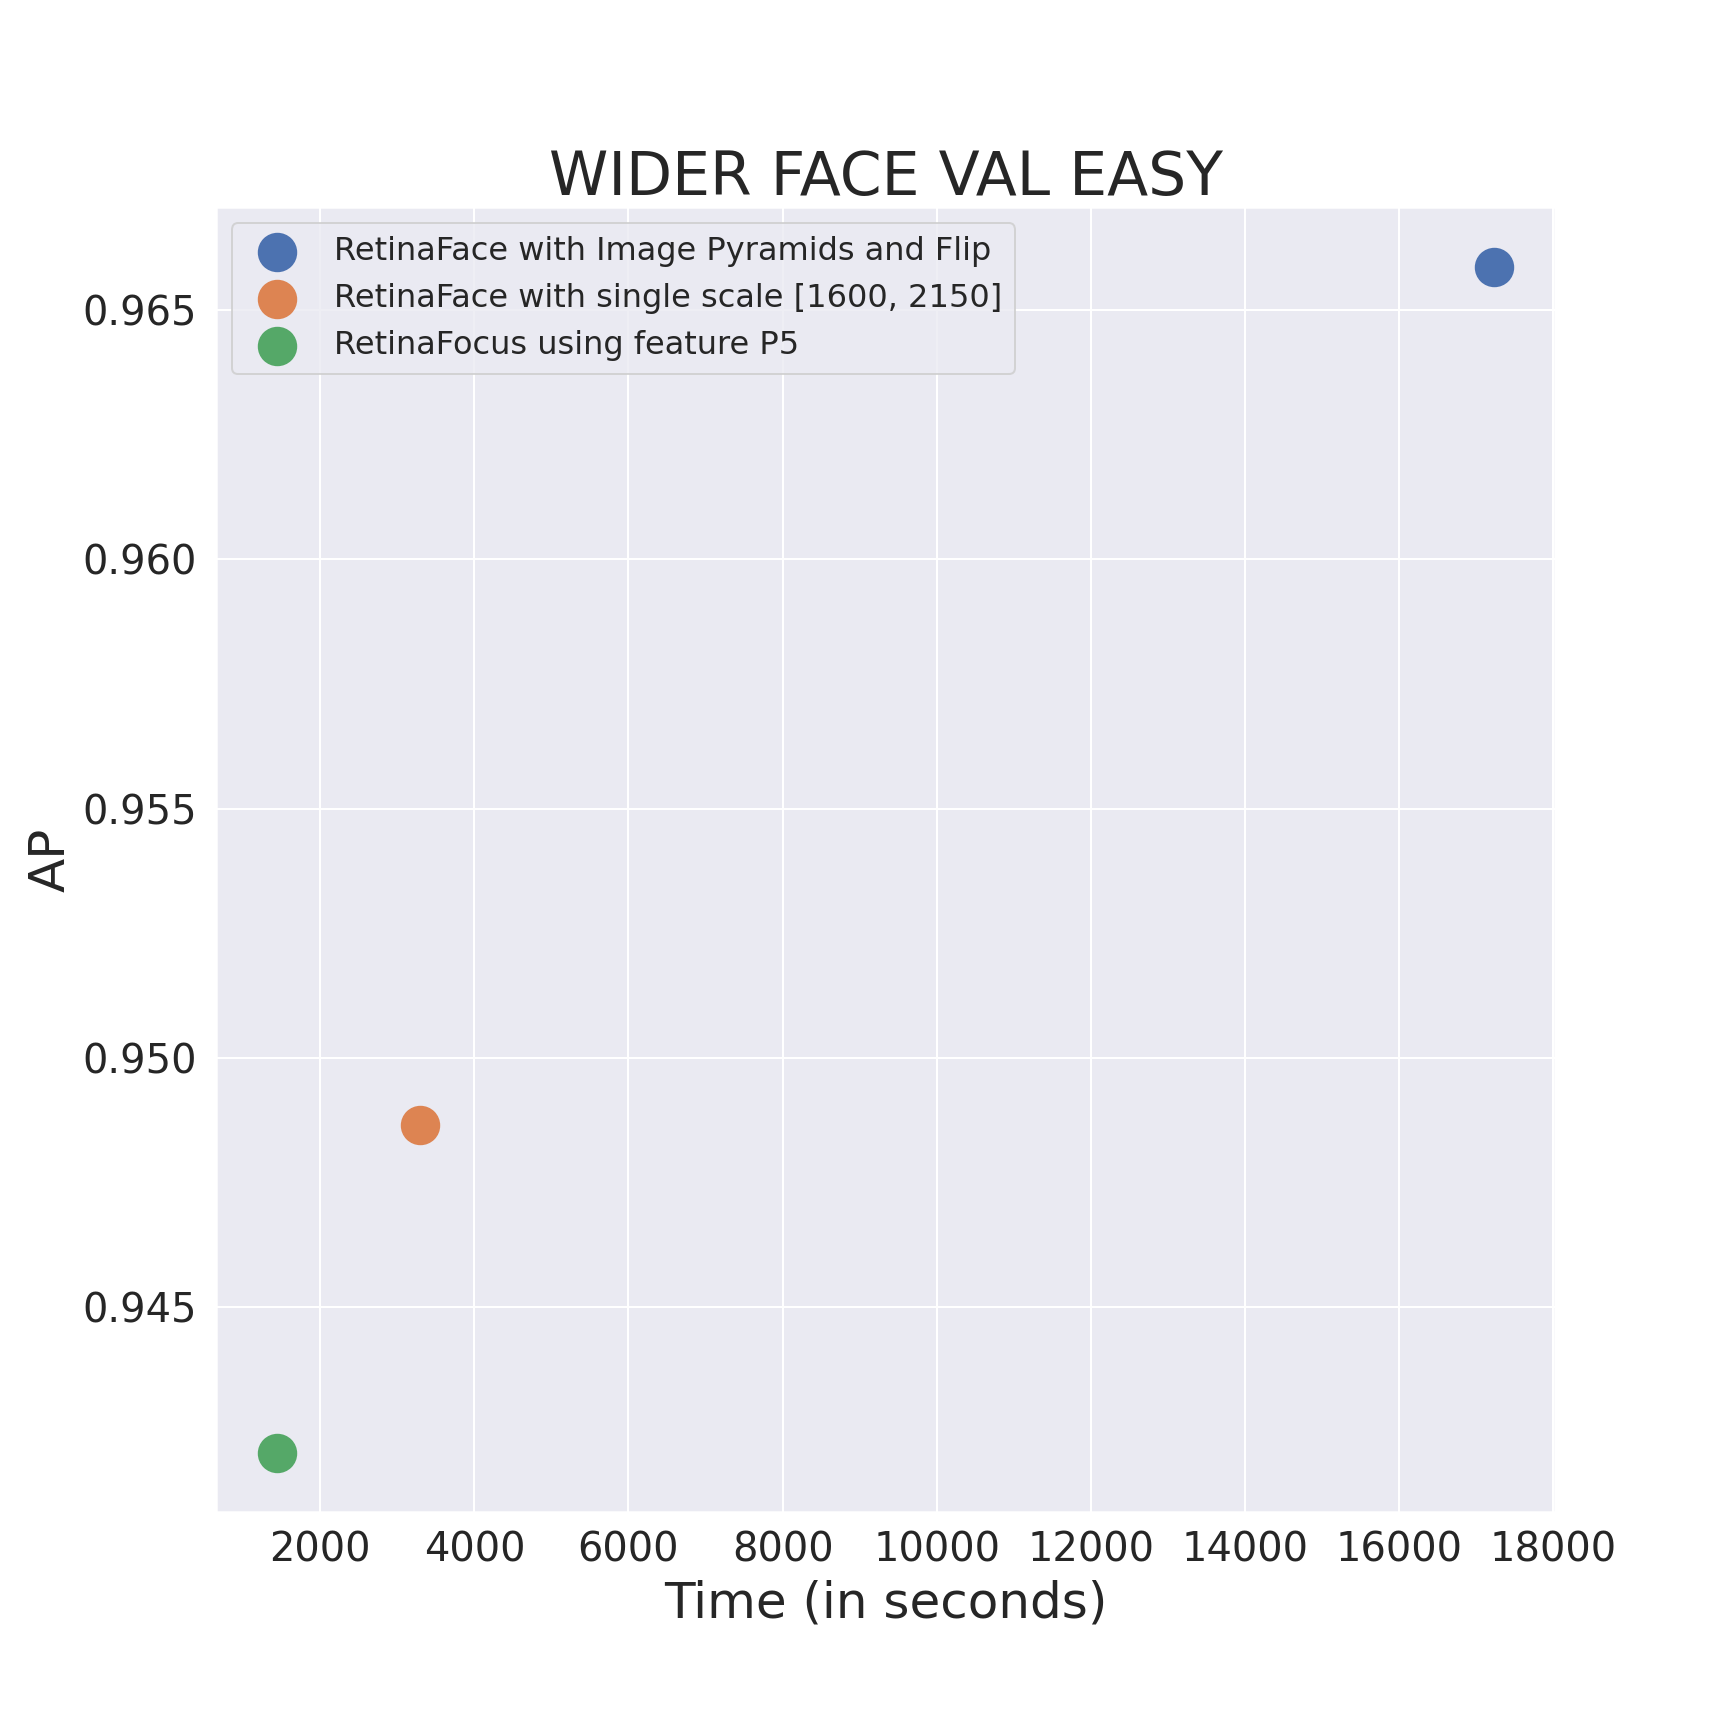
\includegraphics[width=7.3cm]{images/retinafocus_widerface_val_easy_rtnf}} 
        \subfigure[]{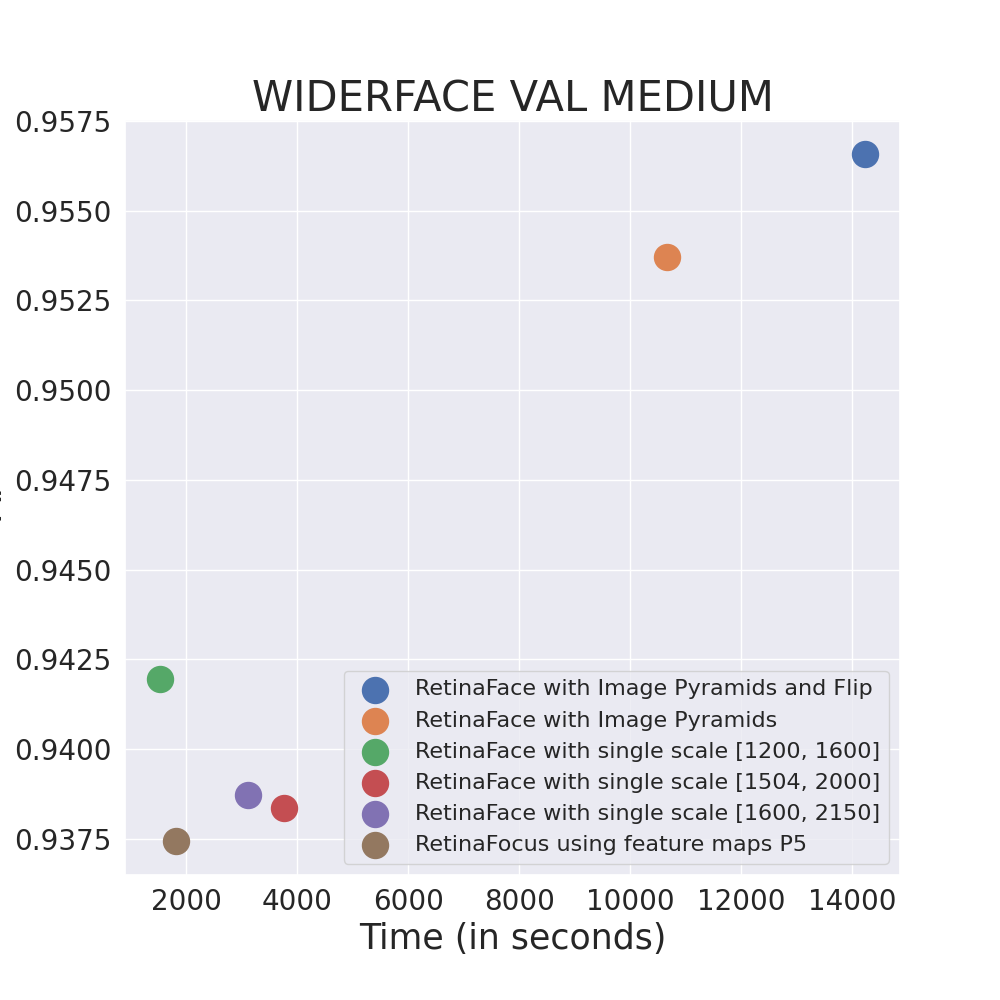
\includegraphics[width=7.3cm]{images/retinafocus_widerface_val_medium_rtnf}} 
        \subfigure[]{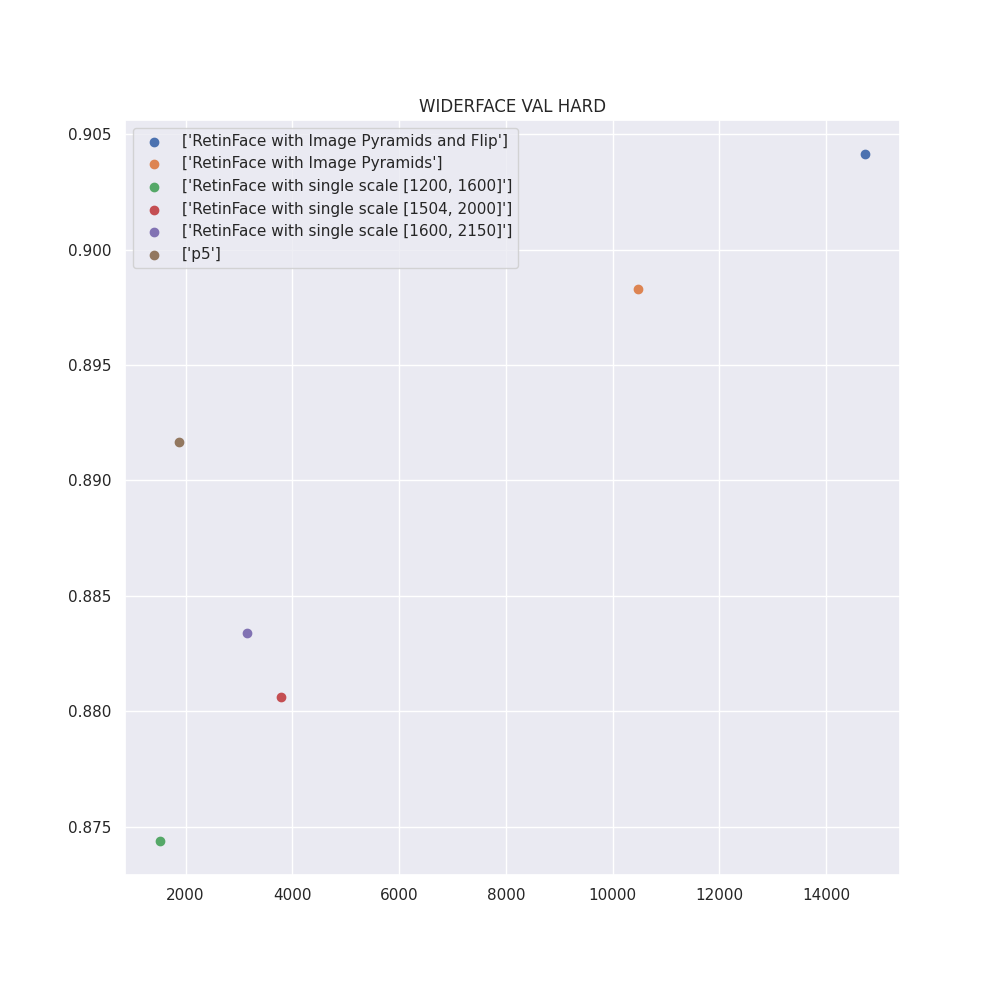
\includegraphics[width=7.3cm]{images/retinafocus_widerface_val_hard_rtnf}} 
        \caption{Kết quả so sánh cấu hình tốt nhất của RetinaFocus với các cấu hình của RetinaFace trên ba bộ dữ liệu WIDER FACE val easy (a), medium (b) và hard (c)}
        \label{fig:retinafocus_widerface_val_rtnf}
    \end{figure}

    Các cấu hình của mô hình RetinaFace sử dụng trong thí nghiệm này bao gồm: \\
    - Cấu hình sử dụng chiến lược Image Pyramids kết hợp với việc lật ảnh đầu vào trong quá trình dự đoán, ký hiệu là \textit{RetinaFace with Image Pyramids and Flip}. \\
    - Cấu hình chỉ sử dụng chiến lược Image Pyramids, ký hiệu là \textit{RetinaFace with Image Pyramids}. \\
    - Cấu hình không sử dụng chiến lược Image Pyramids mà chỉ sử dụng một scale ảnh duy nhất là [1200, 1600], ký hiệu là \textit{RetinaFace with single scale [1200, 1600]}. \\
    - Cấu hình không sử dụng chiến lược Image Pyramids mà chỉ sử dụng một scale ảnh duy nhất là [1504, 2000], ký hiệu là \textit{RetinaFace with single scale [1504, 2000]}. \\
    - Cấu hình không sử dụng chiến lược Image Pyramids mà chỉ sử dụng một scale ảnh duy nhất là [1600, 2150], ký hiệu là \textit{RetinaFace with single scale [1600, 2150]}. \\
    Cấu hình của mô hình RetinaFocus sử dụng trong thí nghiệm này là cấu hình sử dụng bản đồ đặc trưng\index{bản đồ đặc trưng} $P_5$ được ký hiệu là \textit{using feature maps P5}.

    % \begin{figure}[H]
    %     \centering
    %     \subfigure[]{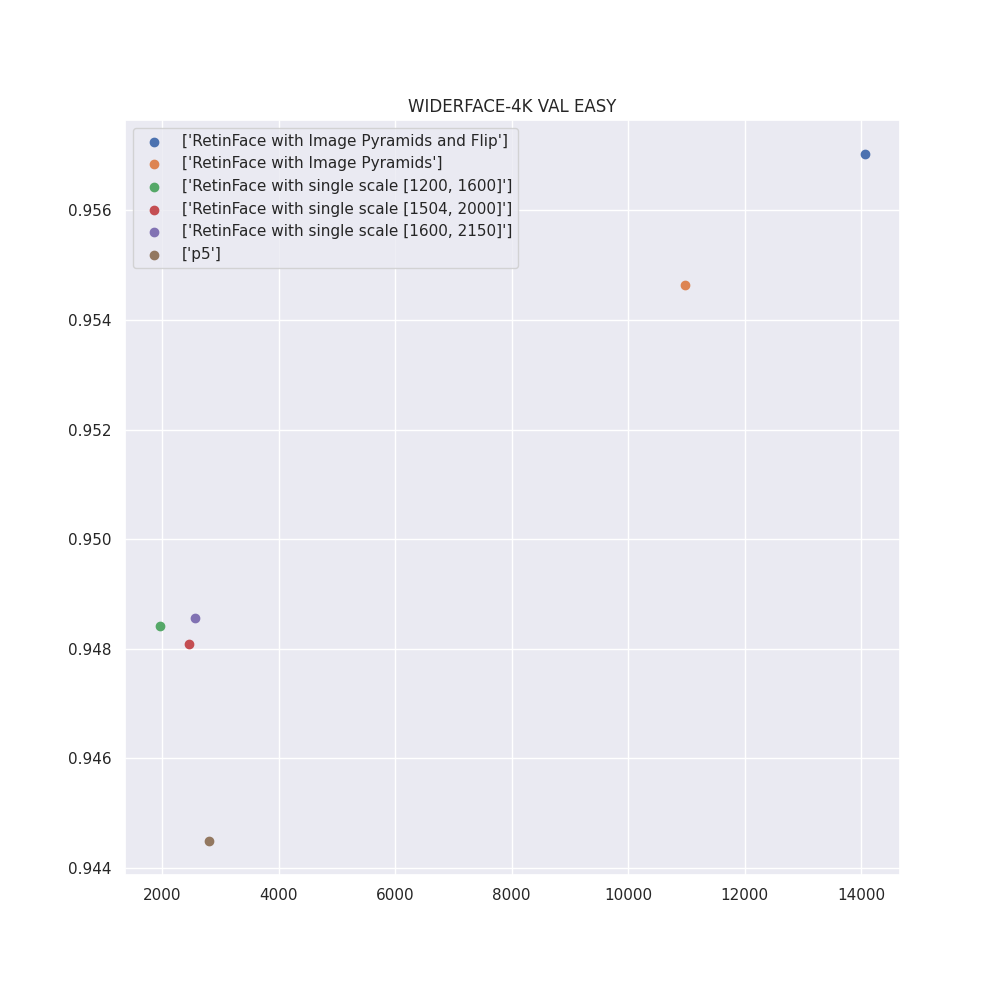
\includegraphics[width=7.3cm]{images/retinafocus_widerface_4k_val_easy_rtnf}} 
    %     \subfigure[]{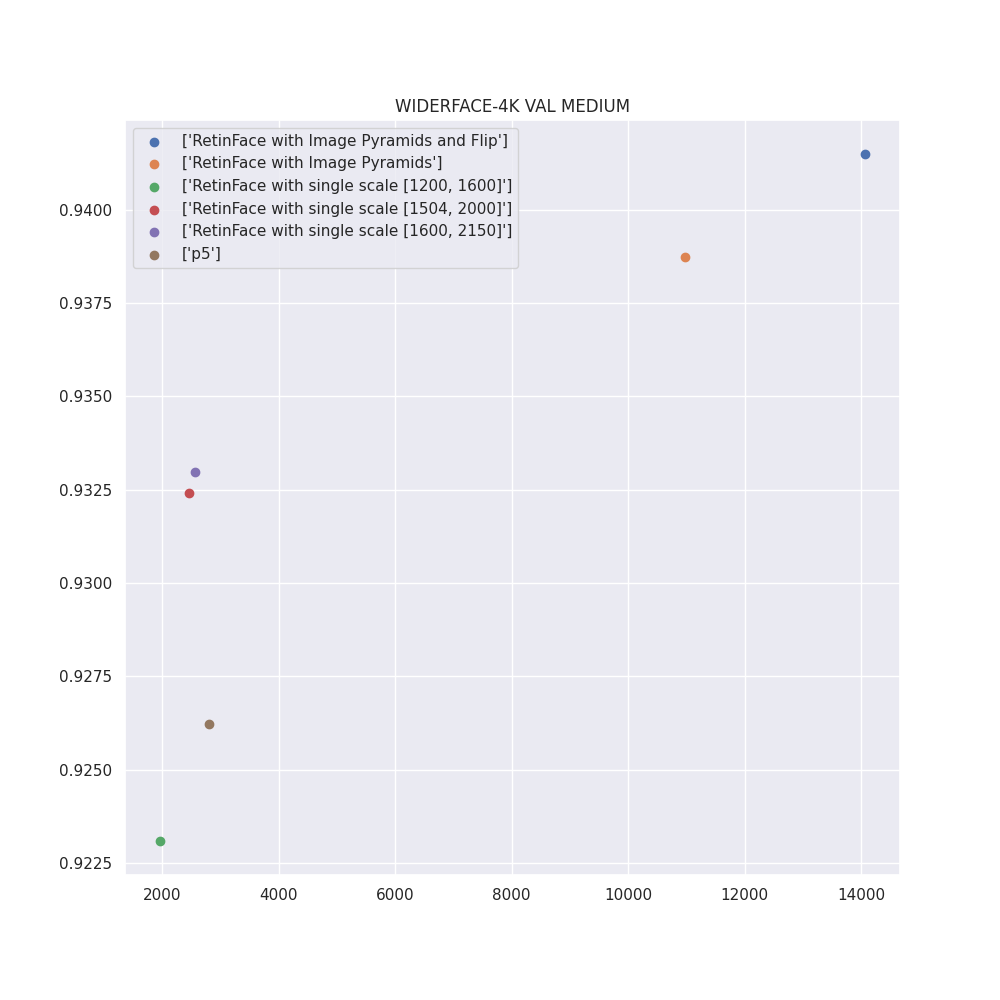
\includegraphics[width=7.3cm]{images/retinafocus_widerface_4k_val_medium_rtnf}} 
    %     \subfigure[]{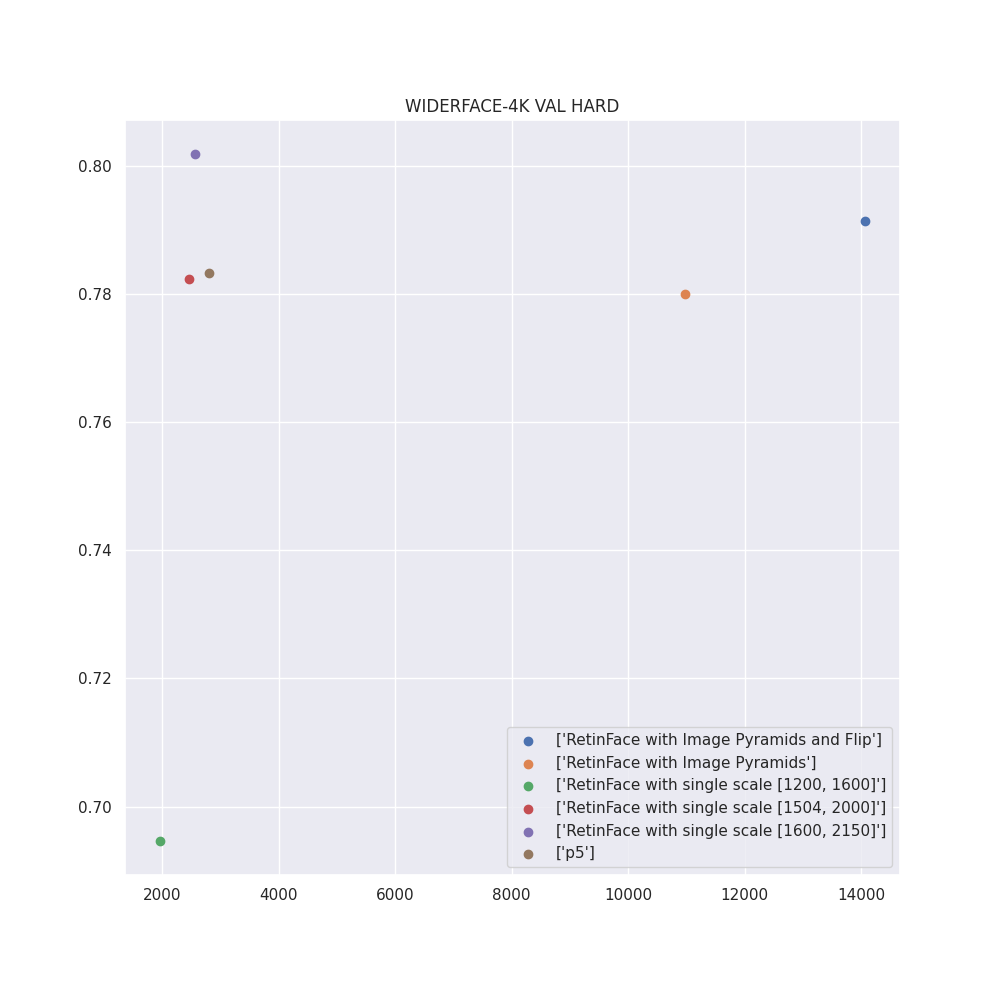
\includegraphics[width=7.3cm]{images/retinafocus_widerface_4k_val_hard_rtnf}} 
    %     \caption{Kết quả so sánh cấu hình tốt nhất của RetinaFocus với các cấu hình của RetinaFace trên ba bộ dữ liệu WIDER FACE 4K val easy (a), medium (b) và hard (c)}
    %     \label{fig:retinafocus_widerface_val_rtnf}
    % \end{figure}

    \noindent
    Trên cả hai bộ dữ liệu WIDER FACE và WIDER FACE 4K của mô hình RetinaFocus đều đạt kết quả cạnh tranh với mô hình RetinaFace nguyên bản trong khi duy trì được tốc độ tốt hơn khá nhiều so với mô hình RetinaFace nguyên bản.
}